% !TeX program = latexmk
% !TeX root = main.tex
%%%%%%%%%%%%%%%%%%%%%%%%%%%%%%%%%%%%%%%%%%%%%%%%%%%%%%%%%%%%%%%%%%%%%%%%%%%%%%%%
% ICRA 2027 paper skeleton, organized like reference/RAL_dexsafedagger.

\documentclass[letterpaper,10pt,conference]{ieeeconf}

% Core writing, math, figure, and table packages. Add specialized packages only
% when the paper needs them; this keeps the submission easier to reproduce.
\usepackage[T1]{fontenc}
\usepackage{amsmath,amssymb,bm}
\usepackage{algorithm,algorithmic}
\usepackage{booktabs,colortbl,multirow,tabularx}
\usepackage{capt-of}
\usepackage[noadjust]{cite}
\usepackage{graphicx}
\usepackage{microtype}
\usepackage{needspace}
\usepackage{siunitx}
\usepackage{tikz}
\usepackage{xcolor}
\usepackage{xspace}
\usepackage{url}
\usetikzlibrary{arrows.meta,positioning}

\graphicspath{{figures/}}

% PaperCept prefers Acrobat 5 / PDF 1.4 compatibility.
\pdfminorversion=4
\pdfobjcompresslevel=0

\IEEEoverridecommandlockouts
\overrideIEEEmargins

% Project macros: rename the method once here and use \methodname throughout.
\newcommand{\methodname}{NUTS\xspace}
\newcommand{\figref}[1]{Fig.~\ref{#1}}
\newcommand{\secref}[1]{Sec.~\ref{#1}}
\newcommand{\tabref}[1]{Table~\ref{#1}}
\newcommand{\etal}{\emph{et al.}\xspace}

% Keep this true for review. Set it false only for a version where ICRA
% explicitly requests identities, such as the camera-ready paper.
\newif\ificraanonymous
\icraanonymoustrue

\title{\LARGE \bfseries
  NUTS: Learning Long-Horizon Cyclic Nut Threading via Hybrid-Teacher
  Policy Distillation
}

\ificraanonymous
  % Preserve the template's byline spacing without exposing author identity.
  \author{\vphantom{Author Names}\\\vphantom{Author Affiliations}}
\else
  \author{Chi Zhang, Carsten Oertel, Lei Zhang, Zhenshan Bing, and Alois Knoll}
\fi

% Match the reference paper's page-one structure: title, a full-width teaser,
% then the two-column abstract and introduction.
\newcommand{\teasercaption}{%
  \textbf{Overview of \methodname---decompose during data collection, unify at
  deployment.} During data collection, an RL policy executes approach, grasp,
  rotate, and goal reaching, while scripted controllers execute release and
  return\&reset; together, they form a hybrid teacher for generating
  long-horizon threading demonstrations. Human corrections augment real-world
  replays to address the sim-to-real gap. Policy distillation then unifies these
  demonstrations into a single visuomotor policy that executes the complete
  cyclic task at deployment.}

\makeatletter
\let\icra@originalmaketitle\@maketitle
\renewcommand{\@maketitle}{%
  \icra@originalmaketitle
  \begin{center}
    
\includegraphics[width=\linewidth,trim=17bp 85bp 5bp 117bp,clip]{%
      figures/SimThreadTeaser.pdf}
    \captionof{figure}{\teasercaption}
    \label{fig:teaser}
    \vspace{-0.12in}
  \end{center}%
}
\makeatother

\begin{document}

\maketitle
% ieeeconf measures the custom title block more than once; normalize the teaser
% counter so the next figure is Fig. 2.
\setcounter{figure}{1}
\thispagestyle{empty}
\pagestyle{empty}

\begin{abstract}
Learning controlled nut threading is one of the most challenging problems in
robotic assembly. Repetitive phases---including grasping, turning, goal
reaching, and release-and-reset---must transition seamlessly to sustain
consecutive threading cycles, making the task long-horizon and sensitive to
errors at phase boundaries. We found that learning all phases end to end with a
single reinforcement-learning policy makes long-horizon reward shaping and
training difficult.
We therefore present \methodname, which follows a simple principle: decompose
during data generation, unify during deployment. A hybrid teacher combines a
privileged RL policy for approach through goal reaching with scripted
release-and-reset behaviors to generate complete multi-cycle demonstrations.
Sparse human corrections augment real-world replays to reduce the sim-to-real
gap. We distill the combined data into a single conditional
flow-matching visuomotor student that predicts eight-step action chunks from
point-cloud features converted from RGB-D observations and executes the full task autonomously.
We evaluate the student policy in
10-cycle trials using in-distribution M24, M30, and M36 hexagonal nuts and
unseen rectangular, octagonal, and round nut geometries. For all
in-distribution nuts, the policy completes all 10 cycles, with mean cyclic
tracking errors below $6^\circ$ in magnitude. Generalization is geometry dependent:
the policy completes all 10 cycles on the round and octagonal
profiles with comparable errors, but barely succeeds on rectangular profiles,
indicating a limitation when test geometry does not support the learned
grasping skill.
\end{abstract}

\section{Introduction}
\label{sec:introduction}
% !TeX root = main.tex
Multi-fingered, contact-rich manipulation over long execution horizons remains
one of the open frontiers of real-world robotics~\cite{siciliano2016springer}.
Tasks such as threading a nut onto a bolt are effortless for humans yet expose
the full difficulty of autonomous dexterity: the robot must regulate motion
through sustained contact under tight geometric tolerances, uncertain friction,
and only partially observed interaction forces. Small pose errors cause
slipping, jamming, or cross-threading, while excessive force damages the
workpiece. These tightly coupled perception, control, and contact constraints
make controlled threading one of the most demanding contact-rich manipulation
problems, and its difficulty is compounded when a dexterous hand, rather than a
parallel gripper, must coordinate many degrees of freedom to sustain
engagement.

The difficulty grows sharply over long horizons. Because the reachable rotation
of a wrist or hand is bounded, a single continuous turn cannot fully seat a nut;
the operation instead requires a \emph{cyclic} sequence of partial rotations,
timely release, collision-free return, and re-engagement, repeated until the nut
is fully threaded. This cyclic structure is what turns a short-horizon contact
skill into a long-horizon task: the terminal state of each cycle is the initial
condition of the next, so a small deviation in one rotation perturbs contact in
the following one. Under closed-loop autoregressive execution such deviations
accumulate, driving the policy toward out-of-distribution states from which
recovery is unlikely---the compounding-error, or covariate-shift, failure mode
that is well understood in imitation learning~\cite{ross2011reduction}. Purely
scripted trajectories cannot react to these deviations, while a monolithic
learned policy must simultaneously discover fine contact behavior and the
long-horizon phase transitions that stitch cycles together.

Sim-to-real reinforcement learning with privileged information has become the
dominant recipe for short-horizon contact-rich skills. High-fidelity contact
simulators built on signed-distance-field (SDF) collision
representations~\cite{narang2022factory} enable stable, fast simulation of tight
assembly, and force-aware policies trained under dynamics randomization transfer
robustly to hardware for tasks including insertion, gear meshing, and single
nut threading~\cite{noseworthy2025forge}. However, these successes are largely
confined to short contact episodes. When the same recipe is scaled to complex
dexterous assets and long horizons, two failure modes emerge. First, residual
gaps in contact and friction modeling let a reinforcement-learning agent
\emph{exploit} simulator inaccuracies rather than learn behavior that survives
the sim-to-real gap---a pathology observed precisely in dexterous nut
screwing~\cite{dexscrew}. Second, the trajectory drift described above turns
otherwise reliable per-cycle policies into unreliable long-horizon ones.

The conventional remedy for long horizons is \emph{policy chaining}:
decomposing the task into discrete sub-skills and learning to transition between
them. Sequential Dexterity~\cite{chen2023sequential}, the representative
approach, chains several reinforcement-learning sub-policies using a learned
transition-feasibility function. This modular design is expressive, but it
carries structural costs that are particularly acute for a cyclic task: it
requires training and maintaining multiple networks, hand-designing or learning
the transition boundaries between them, and absorbing the boundary failures and
execution latency that arise whenever control is handed from one sub-policy to
the next. For a task whose sub-skills are nearly identical and must repeat many
times, replicating this discrete machinery per cycle is both wasteful and a new
source of compounding boundary error.

We argue that the cyclic structure of threading is better captured by a single
\emph{continuous} generative policy than by a chain of discrete ones. We
introduce \methodname, a framework that distills a privileged simulation
teacher into a unified vision-and-force flow-matching student for long-horizon
cyclic threading (\figref{fig:teaser}). We first train a reactive teacher in a
simplified simulation that preserves the SDF-based contact interactions
essential to threading while removing irrelevant complexity, giving the teacher
access to privileged state, contact forces, and exact geometry. Because a single
reachable rotation is bounded, we generate long-horizon demonstrations by rolling
out this \emph{single} reactive teacher inside a state machine: the policy
threads until a rotation threshold is reached, a guided open-and-return motion
then resets the hand to its initial opened configuration, and the same policy is
re-invoked to thread the next increment in the same environment. Repeating this
cycle produces arbitrarily long demonstrations without ever switching between
distinct learned sub-policies. We then distill these long-horizon rollouts into a
single student policy that replaces privileged state with a DP3 point-cloud
vision head~\cite{ze2024dp3} and force feedback, and that models the full cyclic
trajectory distribution with flow-matching imitation
learning~\cite{lipman2023flow}. Flow matching is well suited to this setting:
it regresses a straight, deterministic velocity field between noise and expert
actions, yielding a multi-modal yet efficient trajectory generator that captures
long-horizon behavior in a single network. Crucially, the deployed student is
\emph{one} continuous policy---it reproduces the entire multi-cycle chain
without switching between discrete sub-networks at runtime, so it avoids the
inter-policy boundary failures and latency of explicit chaining while remaining
reactive to contact.

The main contributions of this work are:
\begin{itemize}
  \item \textbf{System and task.} A hardware platform and benchmark for
    long-horizon cyclic nut threading on a 7-DoF arm equipped with a
    multi-fingered dexterous hand, exercising force-regulated contact over many
    rotation--release--return--re-engage cycles.
  \item \textbf{Privileged flow-matching distillation.} A teacher-to-student
    pipeline that trains a privileged reactive teacher in a simplified
    SDF-contact simulation and distills its long-horizon behavior into a single
    flow-matching policy, rather than a chain of learned sub-policies.
  \item \textbf{Cross-modal sim-to-real integration.} A student policy that
    substitutes a DP3 visual-latent representation and force feedback for the
    teacher's privileged simulation state, transferring contact-rich behavior to
    the real world without runtime policy switching.
  \item \textbf{Empirical validation.} An evaluation across M24, M30, and M36
    nuts with hexagonal, octagonal, rectangular, and round geometries, reporting
    maximum cycle count, threading tracking error, and success rate to quantify
    robustness and generalization.
\end{itemize}


\section{Related Work}
\label{sec:related_work}
% Declare the two-column method overview early so it appears one page sooner.
\begin{figure*}[t]
  \centering
  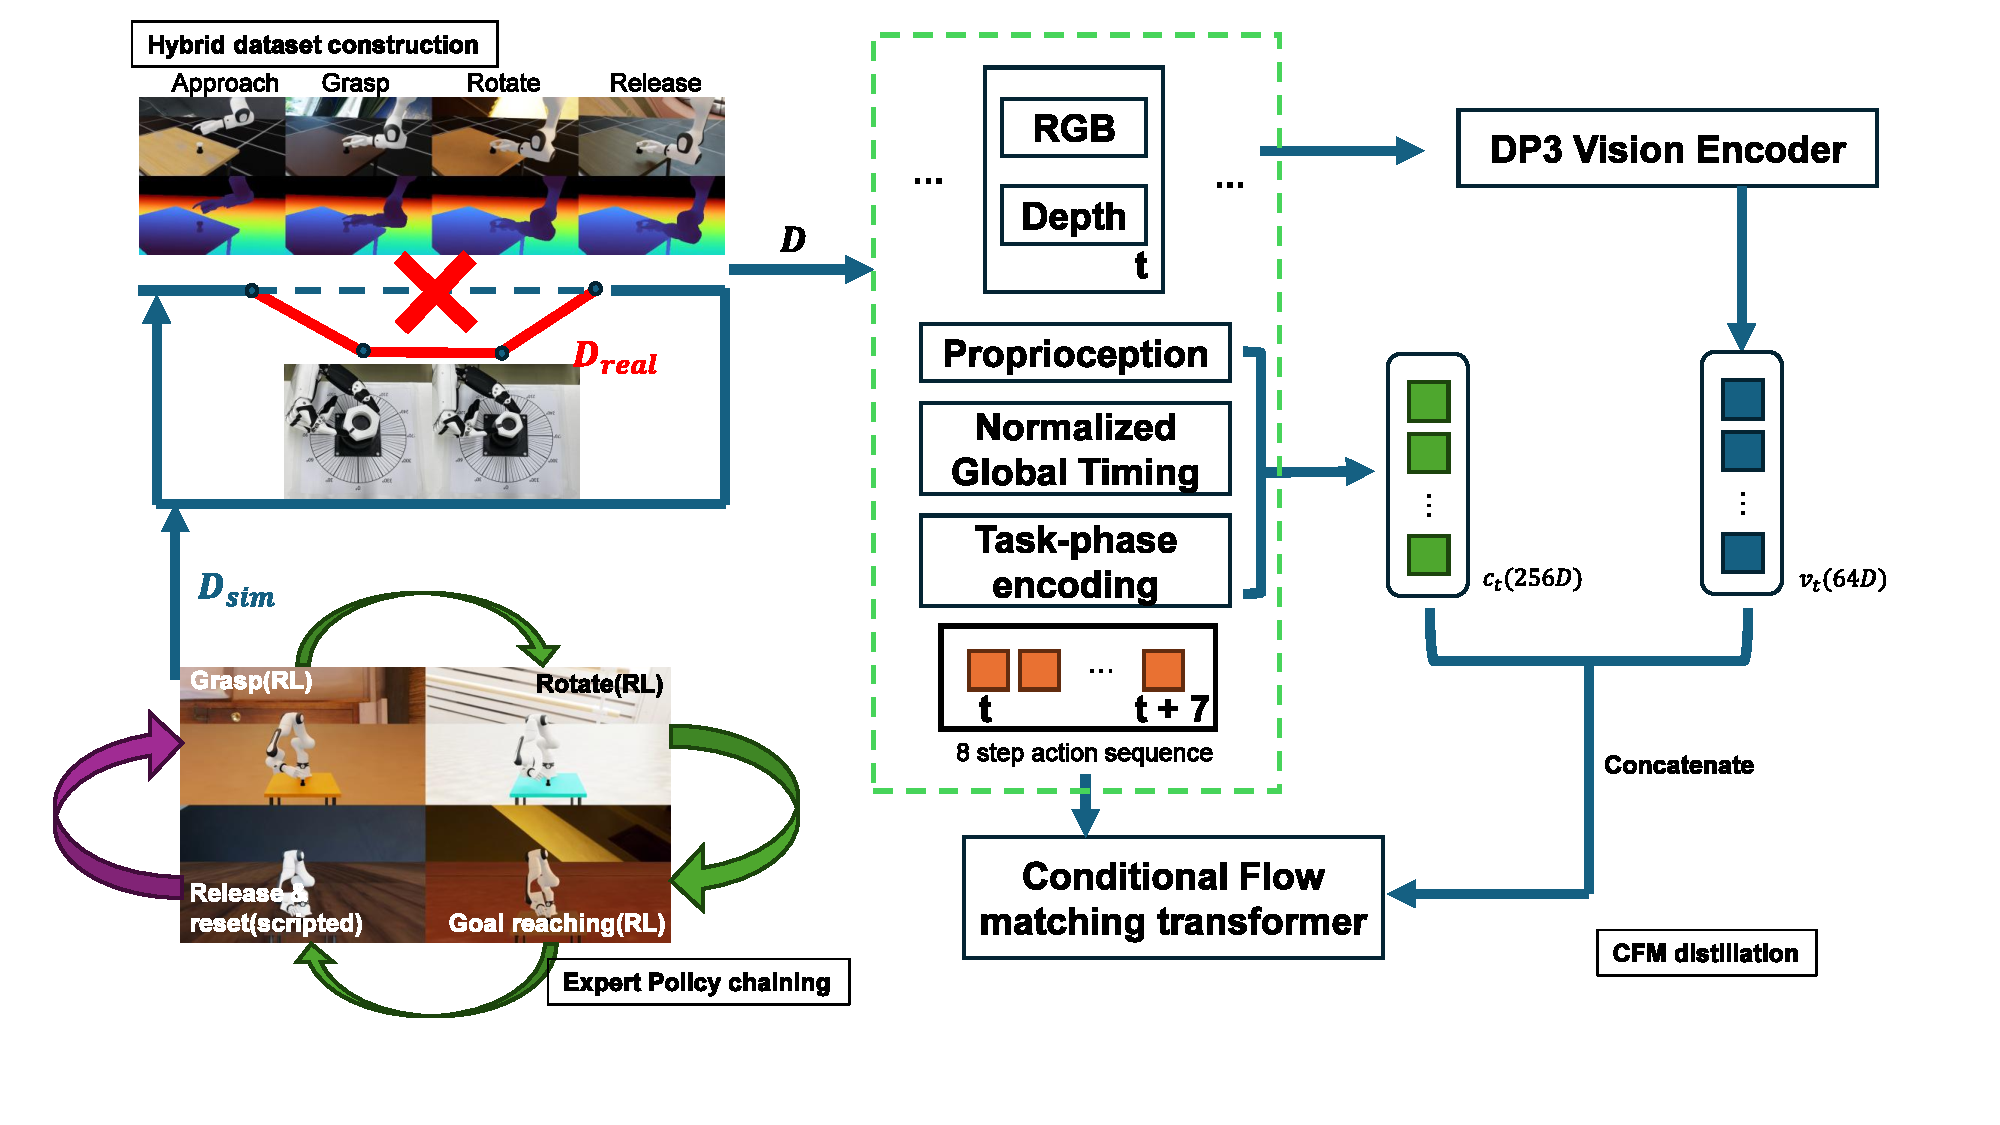
\includegraphics[width=0.90\textwidth]{mainpipeline.pdf}
  \caption{Detailed NUTS pipeline. An RL teacher is repeatedly rolled out with
    a scripted policy to construct cyclic threading demonstrations in
    simulation; together, they form the hybrid teacher. During real-world
    replay, human corrections replace flawed trajectory segments from grasp
    through release, forming a mixed simulation and real-world dataset. The
    conditional flow-matching student takes a 64-D visual feature extracted by
    a DP3 vision encoder from RGB-D observations and a 256-D state feature
    comprising proprioception, timing, and phase encodings, and predicts an
    eight-step action chunk.}
  \label{fig:main_pipeline}
\end{figure*}

% !TeX root = main.tex
\textbf{First research area.}
Summarize the literature most directly connected to the task, grouping papers
by technical idea instead of listing them chronologically.

\textbf{Second research area.}
Explain how the proposed work differs from the closest prior approaches. Make
the unresolved limitation precise enough to motivate the method in
\secref{sec:method}.


\section{Problem Statement and Method}
\label{sec:method}
% !TeX root = main.tex
\begin{figure*}[t]
  \centering
  \resizebox{\linewidth}{!}{% Full-width method/pipeline placeholder. Replace with a PDF figure when ready.
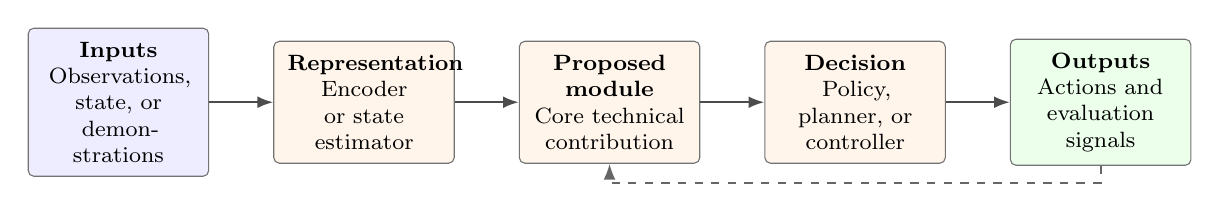
\begin{tikzpicture}[
  font=\footnotesize,
  module/.style={
    draw=black!55,
    rounded corners=2pt,
    minimum height=0.58in,
    text width=0.16\textwidth,
    align=center,
    inner sep=5pt
  },
  flow/.style={-{Latex[length=2mm]}, line width=0.75pt, draw=black!70},
  feedback/.style={-{Latex[length=2mm]}, dashed, line width=0.7pt, draw=black!60}
]
  \node[module, fill=blue!7] (input) {\textbf{Inputs}\\Observations, state, or demonstrations};
  \node[module, fill=orange!8, right=0.32in of input] (representation) {\textbf{Representation}\\Encoder or state estimator};
  \node[module, fill=orange!8, right=0.32in of representation] (method) {\textbf{Proposed module}\\Core technical contribution};
  \node[module, fill=orange!8, right=0.32in of method] (decision) {\textbf{Decision}\\Policy, planner, or controller};
  \node[module, fill=green!8, right=0.32in of decision] (output) {\textbf{Outputs}\\Actions and evaluation signals};

  \draw[flow] (input) -- (representation);
  \draw[flow] (representation) -- (method);
  \draw[flow] (method) -- (decision);
  \draw[flow] (decision) -- (output);
  \draw[feedback] (output.south) -- ++(0,-0.22) -| (method.south);
\end{tikzpicture}
}
  \caption{Placeholder for the full method or system pipeline. Replace each
    block with a meaningful stage, show the direction of data flow, and explain
    train-time versus deployment-time components in the caption.}
  \label{fig:pipeline}
\end{figure*}

\subsection{Problem Formulation}

Define the task, assumptions, and notation before describing the method. For a
state $\mathbf{x}_t$ and control $\mathbf{u}_t$, a generic discrete-time model is
\begin{equation}
  \mathbf{x}_{t+1} = f(\mathbf{x}_t, \mathbf{u}_t) + \boldsymbol{\varepsilon}_t,
  \label{eq:dynamics}
\end{equation}
where $\boldsymbol{\varepsilon}_t$ denotes process uncertainty. Refer to
equations by label, as in~\eqref{eq:dynamics}.

\subsection{Approach}

Describe enough implementation detail for another researcher to reproduce
\methodname. Use \figref{fig:pipeline} to give the high-level flow before
introducing individual components.

\subsection{Core Components}

Give each novel component its own paragraph or subsection. For every component,
state its inputs, outputs, training signal, and role in the complete system.
Move secondary derivations to concise prose when space is limited.

\begin{algorithm}[t]
  \caption{Placeholder for \methodname training or inference}
  \label{alg:method}
  \begin{algorithmic}[1]
    \REQUIRE Inputs, model components, and stopping condition
    \STATE Initialize the learnable components and data buffers
    \FOR{each training iteration or control step}
      \STATE Observe the current input
      \STATE Compute the proposed intermediate representation
      \STATE Apply the core method and obtain an output
      \STATE Update the model, controller, or stored data if required
    \ENDFOR
    \RETURN Trained model, policy, plan, or action
  \end{algorithmic}
\end{algorithm}



\section{Experiments}
\label{sec:experiments}
% !TeX root = main.tex
\subsection{Evaluation Metrics}

We evaluate performance using two complementary metrics.

\paragraph{Maximum Cycle Count}
The maximum cycle count is the largest number of consecutive task cycles
completed before failure; higher values indicate better long-horizon
robustness.

\paragraph{Threading Tracking Error}
The threading tracking error measures the deviation of the observed thread from
its desired trajectory during execution; lower values indicate more accurate
tracking.

\subsection{Experimental Setup}

We evaluate the proposed method in both simulation and on real hardware using
the metrics defined above. Our platform comprises a seven-DoF Franka Research
3 (FR3) arm equipped with an Inspire Hand RH56DFX. Its simulated counterpart is
implemented in NVIDIA Isaac Sim~5.1.0 with Isaac Lab~2.2.1 and is used for
privileged teacher training, hybrid demonstration generation, and evaluation
before real-world transfer. The simulated and physical systems use the same
task geometry and OSC action interface.

In both settings, the student converts depth observations into cropped point
clouds and discards RGB. An Intel RealSense D415 supplies the physical RGB-D
stream. Real-world evaluation covers three nut sizes---M24, M30, and
M36---and four geometries per size: hexagonal, octagonal, rectangular, and
round.

% TODO: Validate and report the GPU, number of parallel environments, control
% and policy frequencies, camera calibration/resolution/frame rate,
% domain-randomization ranges, workspace and safety limits, trial counts,
% initialization distributions, and success/failure criteria.

\begin{figure}[t]
  \centering
  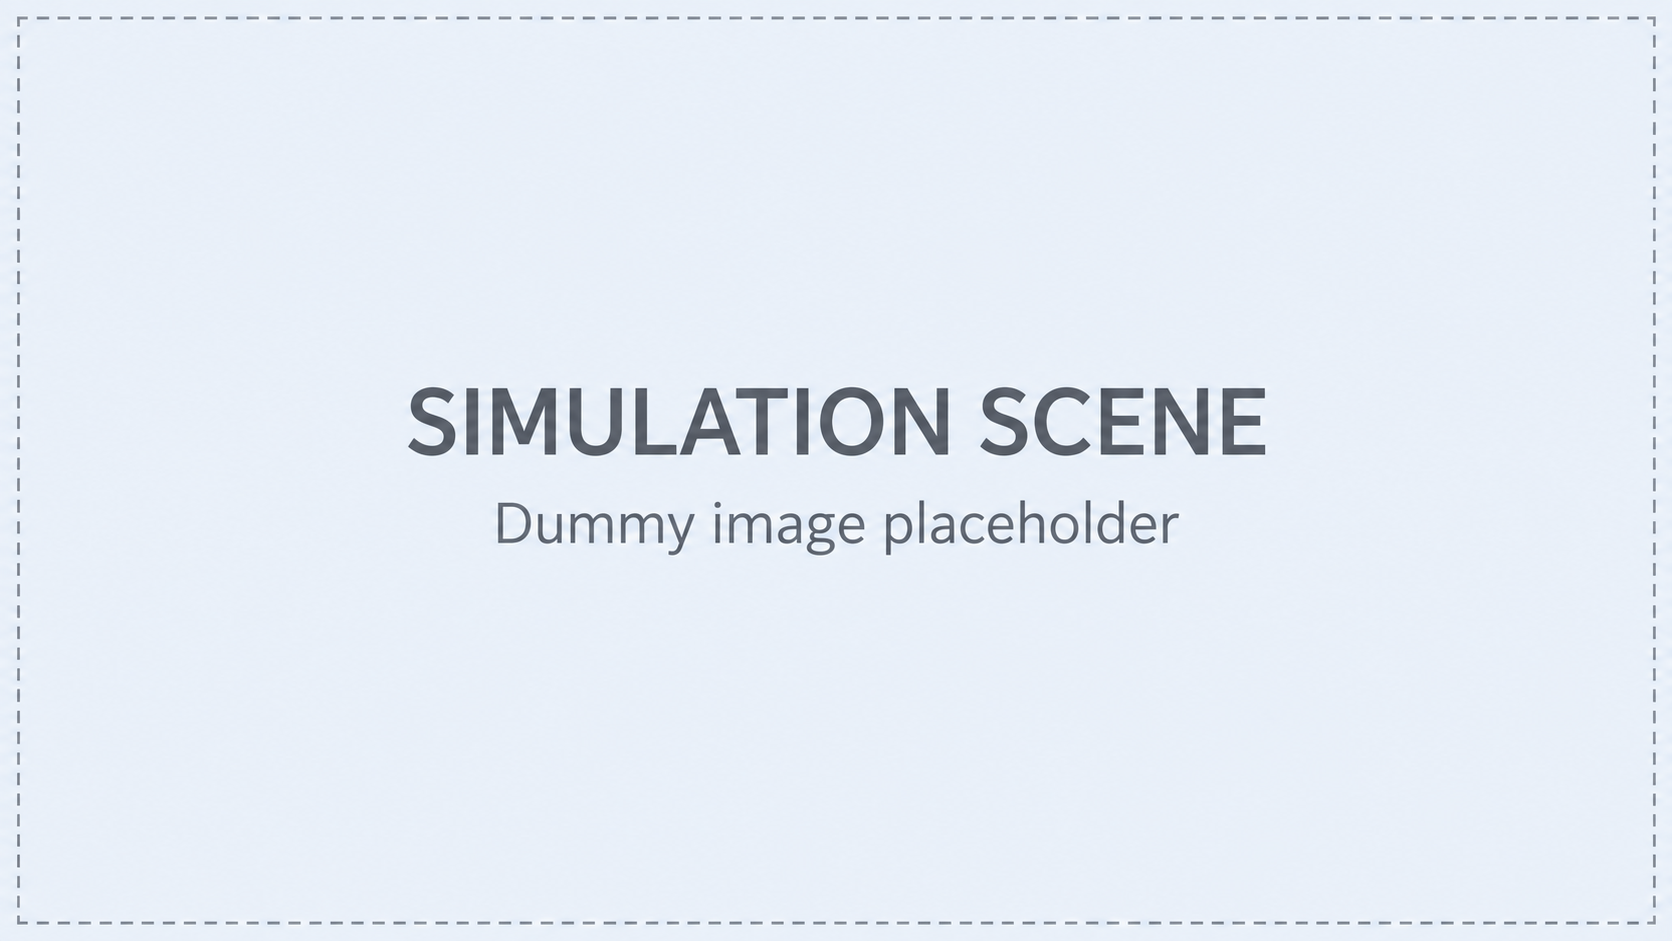
\includegraphics[width=\columnwidth]{figures/simulation_scene_placeholder.png}
  \caption{Simulation scene used for evaluation. Replace this placeholder with
    a representative view of the simulated robot, workspace, and threading
    task.}
  \label{fig:simulation_scene}
\end{figure}

\begin{figure}[t]
  \centering
  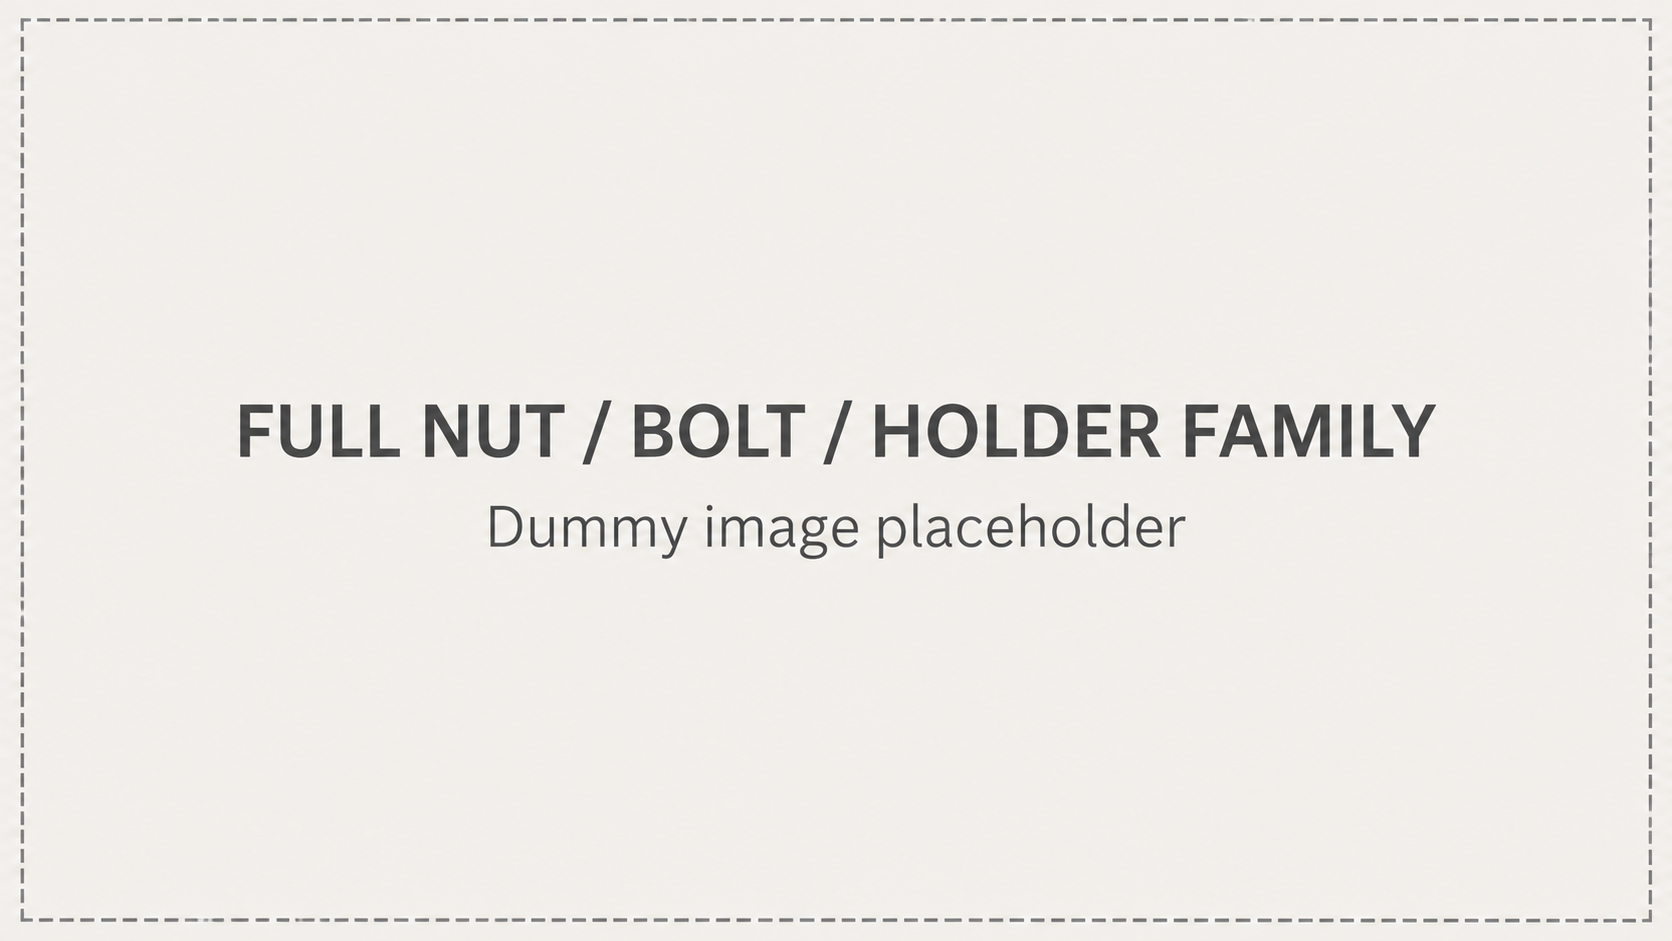
\includegraphics[width=\columnwidth]{figures/hardware_family_placeholder.png}
  \caption{Full family of nuts, bolts, and holders used in the real-hardware
    experiments. Replace this placeholder with a photograph showing all test
    objects and their geometric variations.}
  \label{fig:hardware_family}
\end{figure}

\subsection{Ablations}

We compare four policy-learning variants while keeping the architecture,
dataset budget, evaluation protocol, and all unrelated settings fixed.

\paragraph{Behavior Cloning}
Train the student policy using supervised behavior cloning on the initially
collected teacher demonstrations only.

\paragraph{Online DAgger}
Iteratively execute the current student policy, query the teacher online for
corrective actions on visited states, aggregate the new samples, and retrain the
student policy.

\paragraph{Offline DAgger}
Train on a fixed, pre-collected dataset that includes teacher corrections for
states visited by an intermediate student policy, without additional online
interaction during final training.

\paragraph{Ours}
Train once on the fixed dataset of hybrid-expert demonstrations and offline
human corrections using the proposed flow-matching imitation objective; no
student rollouts or online relabeling are used during training.

\subsection{Quantitative Results}

\begin{table}[htbp]
  \caption{Maximum cycle count for each nut size and geometry. Higher is
    better. Replace dashes with measured values.}
  \label{tab:maximum_cycle_count}
  \centering
  \begin{tabular}{lccc}
    \toprule
    Geometry & M24 & M30 & M36 \\
    \midrule
    Hexagonal  & -- & -- & -- \\
    Octagonal  & -- & -- & -- \\
    Rectangular & -- & -- & -- \\
    Round      & -- & -- & -- \\
    \bottomrule
  \end{tabular}
\end{table}


\begin{table}[htbp]
  \caption{Threading tracking error for each nut size and geometry. Lower is
    better. Replace dashes with measured values and report the unit.}
  \label{tab:thread_tracking_error}
  \centering
  \begin{tabular}{lccc}
    \toprule
    Geometry & M24 & M30 & M36 \\
    \midrule
    Hexagonal  & -- & -- & -- \\
    Octagonal  & -- & -- & -- \\
    Rectangular & -- & -- & -- \\
    Round      & -- & -- & -- \\
    \bottomrule
  \end{tabular}
\end{table}


\begin{table}[htbp]
  \caption{Success rate (\%) for each nut size and geometry. Higher is better.
    Replace dashes with measured values.}
  \label{tab:success_rate}
  \centering
  \begin{tabular}{lccc}
    \toprule
    Geometry & M24 & M30 & M36 \\
    \midrule
    Hexagonal  & -- & -- & -- \\
    Octagonal  & -- & -- & -- \\
    Rectangular & -- & -- & -- \\
    Round      & -- & -- & -- \\
    \bottomrule
  \end{tabular}
\end{table}


Interpret the three comparisons instead of repeating table entries. Discuss
maximum cycle count, threading tracking error, and success rate together, and tie
every central claim to the corresponding table or statistical test.

\subsection{Qualitative and Real-World Results}

Use vector figures (PDF) when possible, and ensure plot text remains legible at
the final column width. Discuss failure cases rather than reporting only the
best outcomes in the quantitative tables.


\section{Conclusion and Future Work}
\label{sec:conclusion}
% !TeX root = main.tex
Summarize the answer to the paper's central question, the strongest supporting
result, and the main limitation. Close with a specific direction for future
work without repeating the abstract.


% Uncomment if an appendix is permitted and fits within the page limit.
% \appendix
% % !TeX root = main.tex
Place optional derivations or implementation details here only if the current
conference rules permit them and the complete paper remains within the page
limit.


% Keep acknowledgments out of anonymous review if they reveal identity.
\ificraanonymous
\else
  \section*{Acknowledgment}
  Add funding and non-author contributions here. Disclose reportable use of
  generative AI according to the current IEEE-RAS policy.
\fi

{\small
  \bibliographystyle{IEEEtran}
  \bibliography{main}
}

\end{document}
